\begin{box_titre}{Polynômes de \textsc{Tchebychev} de première espèce}
    Les polynômes de \textsc{Tchebychev} de première espèce sont les \textbf{uniques} polynômes $(\Tcheby_n)_{n \geqslant 0}$ définis sur $]-1, 1[$ par
    $$\forall \theta \in \R,\ \Tcheby_n (\cos \theta) = \cos(n \theta).$$
\end{box_titre}

\underline{Relation de récurrence:}
$$\boxed{\Tcheby_{n+2} = 2X \Tcheby_{n+1} - \Tcheby_n}$$
Cette relation permet de montrer l'existence de ces polynômes. \\
L'unicité de $\Tcheby_n$ pour $n$ fixé est garantie pas l'identification de \textbf{deux polynômes coïncidant} sur $]-1, 1[$. \\
Les polynômes de \textsc{Tchebychev} forment une famille orthogonale pour le produit scalaire
$$\langle P, Q \rangle = \int_{-1}^{1} P(t) Q(t) \frac{1}{\sqrt{1-t^2}} \d t.$$

\begin{marginfigure}[-8.5cm]
    \centering
	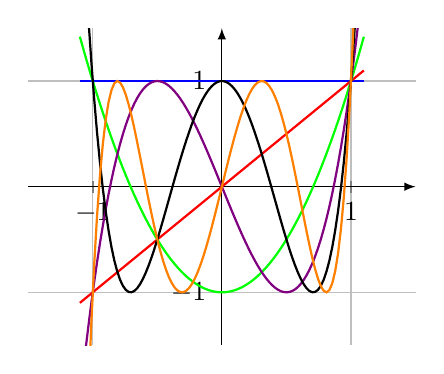
\begin{tikzpicture}
    \begin{axis}[width=6.5cm,
        axis lines=middle,
        inner axis line style={-latex},
        grid=major,
        xmin=-1.5, xmax=1.5,
        ymin=-1.5, ymax=1.5,
        % xlabel=$x$, xlabel style={right},
        % ylabel=$y$, ylabel style={above},
        tick style={thick},
        ticklabel style={font=\normalsize},
        xtick={-1, 0, 1}, 
        ytick={-1, 0, 1},
        % legend entries={0.5x},
            legend style={
            at={(1.05,0.4)},
            anchor=north,
            legend columns=1},
            legend cell align={left}
    ]
    
    \def\a{-1.1}
    \def\b{1.1}
    
    \addplot[blue,thick,samples=100,domain=\a:\b] {1};
    \addplot[red,thick,samples=100,domain=\a:\b] {x};
    \addplot[green,thick,samples=100,domain=\a:\b] {2*x^2-1};
    \addplot[violet,thick,samples=100,domain=\a:\b] {4*x^3-3*x};
    \addplot[black,thick,samples=100,domain=\a:\b] {8*x^4-8*x^2+1};
    \addplot[orange,thick,samples=100,domain=\a:\b] {16*x^5-20*x^3+5*x};
    
   % \legend{$\Leg_0$, 
   %         $\Leg_1$,
%            $\Leg_2$,
%            $\Leg_3$,
 %           $\Leg_4$,
  %          $\Leg_5$
   %         }
    \end{axis}
\end{tikzpicture}
	\caption*{\centering Polynômes de \textsc{Tchebychev} de première espèce}
	{\small
	\color{blue} $$\Tcheby_0 = 1$$
	\color{red} $$\Tcheby_1 = x$$
	\color{green} $$\Tcheby_2 = 2x^2-1$$
	\color{purple} $$\Tcheby_3 = 4x^3-3x$$
	\color{black} $$\Tcheby_4 = 8x^4-8x^2+1$$
	\color{orange} $$\Tcheby_5 = 16x^5-20x^3+5x$$
	}
\end{marginfigure}
